\subsection{Introduction}
\label{rasc:sec:intro}

In the last decade, industry and users have moved away from managing individual IoT (Internet of Things) devices to programming and managing
IoT device {\it collections}. 
IoT permeates our homes~\cite{IoTfuture}, workplaces~\cite{commit.mmsys},  farms~\cite{farmbeats}, Industry 4.0~\cite{lampropoulos2019internet}, entertainment venues~\cite{turchet2018internet}, etc. Smart buildings contain 2 B devices, expected to reach 2.5 B devices and a \$90 B market by 2027, and 4.12 B devices by 2030~\cite{Memoori,memoori2025iot}.
In a single deployment, 10s to 100s of IoT devices may be programmed and managed via automations~\cite{parks2025smarthome} containing a combination of actions~\cite{GHautomations,HAintegrations},
routines~\cite{ifttt,NodeRED},
IFTTT (If This Then That)~\cite{ifttt,reddit_ifttt_2021}, scripts, etc.
An {\it action} is a single command sent to a single device, from a home hub (e.g., Alexa, Google Home hub) or a user device (e.g., phone, tablet, etc.). For instance, the Google Home API~\cite{GHautomations} contains over 50 defined actions, e.g.,  {\tt{blinds.OpenClose}, \tt{SetFanSpeedRelative}, \tt{Cook}, \tt{Dispense}}, etc. 
The most common program written by users is a 
{\it routine}: a sequence of several actions,
which can be triggered conditionally by time, sensors, 
or manually by the user.

\begin{figure}[th]
    \centering
    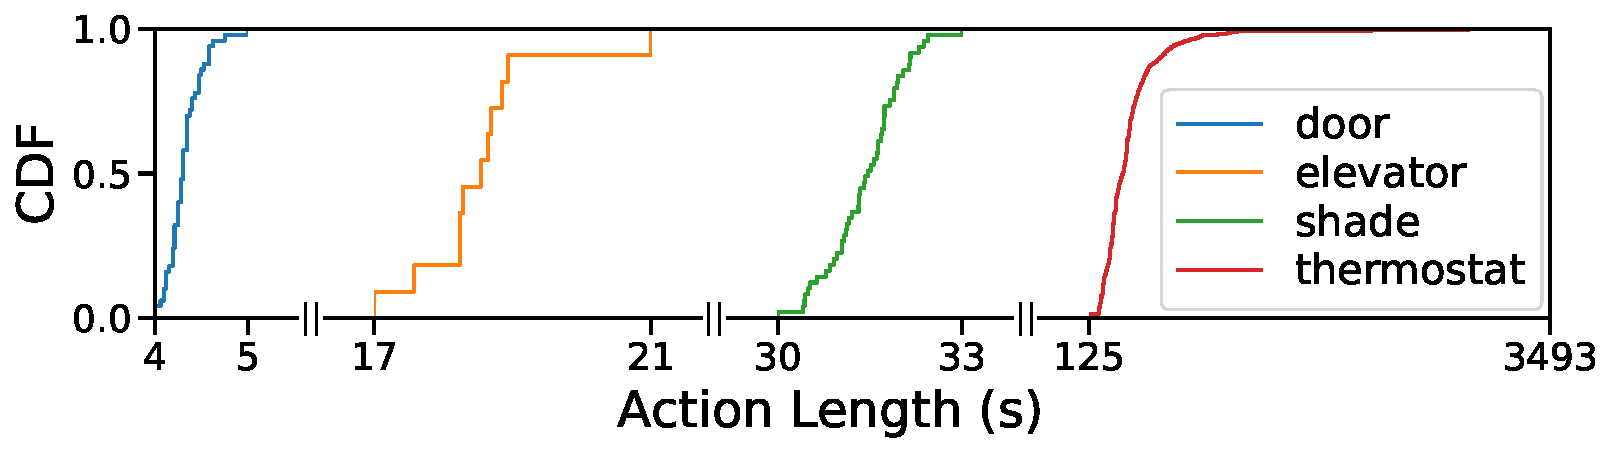
\includegraphics[width=0.7\linewidth]{RASC/figures/intro/action-length-var.pdf}
    \caption{\bf \small IoT actions vary in length. {\it Actions: door: close, elevator: up 1 floor, shade: open, thermostat: heat  68.x to 69.y \textdegree Fahrenheit.} 
    }
    \medskip
    \label{rasc:fig:action-length-variability}
\end{figure}

\noindent \textbf{RPCs and IoT Actions: }
Today, IoT actions
predominantly rely on the traditional RPC (Remote Procedure Call) abstraction~\cite{birrell1984implementing}. 
RPCs are simple, widely understood, and accepted, and have many stock implementations~\cite{grpc,grpc_website,thrift2007,apache_thrift}.
An RPC consists of a single {\it Request} from a hub or
{personal device} towards the IoT device (or its proxy web service), and a single {\it Reply} in the reverse direction.

However, for IoT settings, it is challenging to map the Reply to the appropriate point in the action's execution. 
This is because in user-facing settings like smart spaces, many actions are non-instantaneous, taking seconds or even minutes to execute. 
Physical devices like windows and doors, shades and awnings, kitchen appliances, printers, etc., all 
take several seconds to execute an action (e.g., Google Home API's actions {\tt blinds.OpenClose, SetFanSpeedRelative}). That is, many actions in IoT settings are \textbf{\textit{long actions}}.
Devices like sprinklers, ovens, HVAC systems (heating, ventilation, and air conditioning), etc., may take minutes or hours (e.g., Google Home API's actions {\tt Cook, Dispense,} etc.). Even ``fast'' devices like locks, light bulbs, fans
take a fraction of a second to finish an action. Together, these create a 
non-trivial time gap between starting and completing an action. 
\Cref{rasc:fig:action-length-variability} shows our measurements from devices in our office building. 

Further, there is also a gap between the command's reception and start, due to
\textbf{\textit{preconditions}} for starting a command (e.g., coffee maker's reservoir 
{must have} water). Finally, the \textbf{\textit{action may fail}} (e.g., main door lock is suddenly jammed) and create safety-violating situations. 

Returning to RPCs, 
this diversity in the nature and length of actions in IoT spaces raises the question of {\it which} version of RPC to use. Specifically---{\it when} is the Reply sent back? 
Today's RPC implementations are {\it forced to choose}  mapping of the Reply to one of three choices---either: (1) {\it Acknowledgment}: sent back by the device or its
{cloud} service immediately when it receives the action (we call this {\it \RPCa}), but before the device has started executing the action, {\it or} (2) {\it Start} of the action: sent back by the device or its service when the action starts (we call this {\it \RPCs}), {\it or} (3) {\it Completion} of the action: sent back by the device or its service when the action is completed by the IoT device (we call this {\it \RPCc}). Many commercial smart home deployments today use  \RPCa{} combined with state updates~\cite{Alexa, GoogleHome}, while \RPCc{} is commonly employed in robotics settings~\cite{RECOVER_Cornelio, Zhang_2019_CVPR}. 

\begin{table}[tbh!]
    \centering
    \footnotesize
    % \setlength{\tabcolsep}{1pt} % default is 6pt
    \tagpdfsetup{table/header-rows={1},table/header-columns={1,2}}
    \begin{tabular}{|c|l||c|c|c|c|}
        \hline
        \textbf{Property} & \textbf{Goal} & \textbf{\RPCa} & \textbf{\RPCs} & \textbf{\RPCc} & \textbf{\abstraction} \\ \hline \hline
        \multirow{2}{*}{\it Observability} & Progress updates (\Cref{rasc:sec:adaptive-polling-strategy}) & \xmark & \xmark & \xmark & \cmark \\ \cline{2-6}
        & Failure detection (\Cref{rasc:sec:detect-after-U}) & \xmark & \xmark & $\sim$ & \cmark \\ \hline
        \multirow{2}{*}{\it Programmability} & Diverse dependencies (\Cref{rasc:sec:causality}) & \xmark & \xmark & \xmark & \cmark \\ \cline{2-6}
        & Dynamic scheduling (\Cref{rasc:sec:dyn-sched}) & \xmark & \xmark & $\sim$   & \cmark \\ \hline
    \end{tabular}
    \captionof{table}
    {\bf \small Desired Properties. {\it  $\sim$ means non-trivial design needed.}
    }
    \label{rasc:tab:properties}
\end{table}

\begin{figure}[t]
    \centering
        \begin{subfigure}[b]{\linewidth}
        \centering
        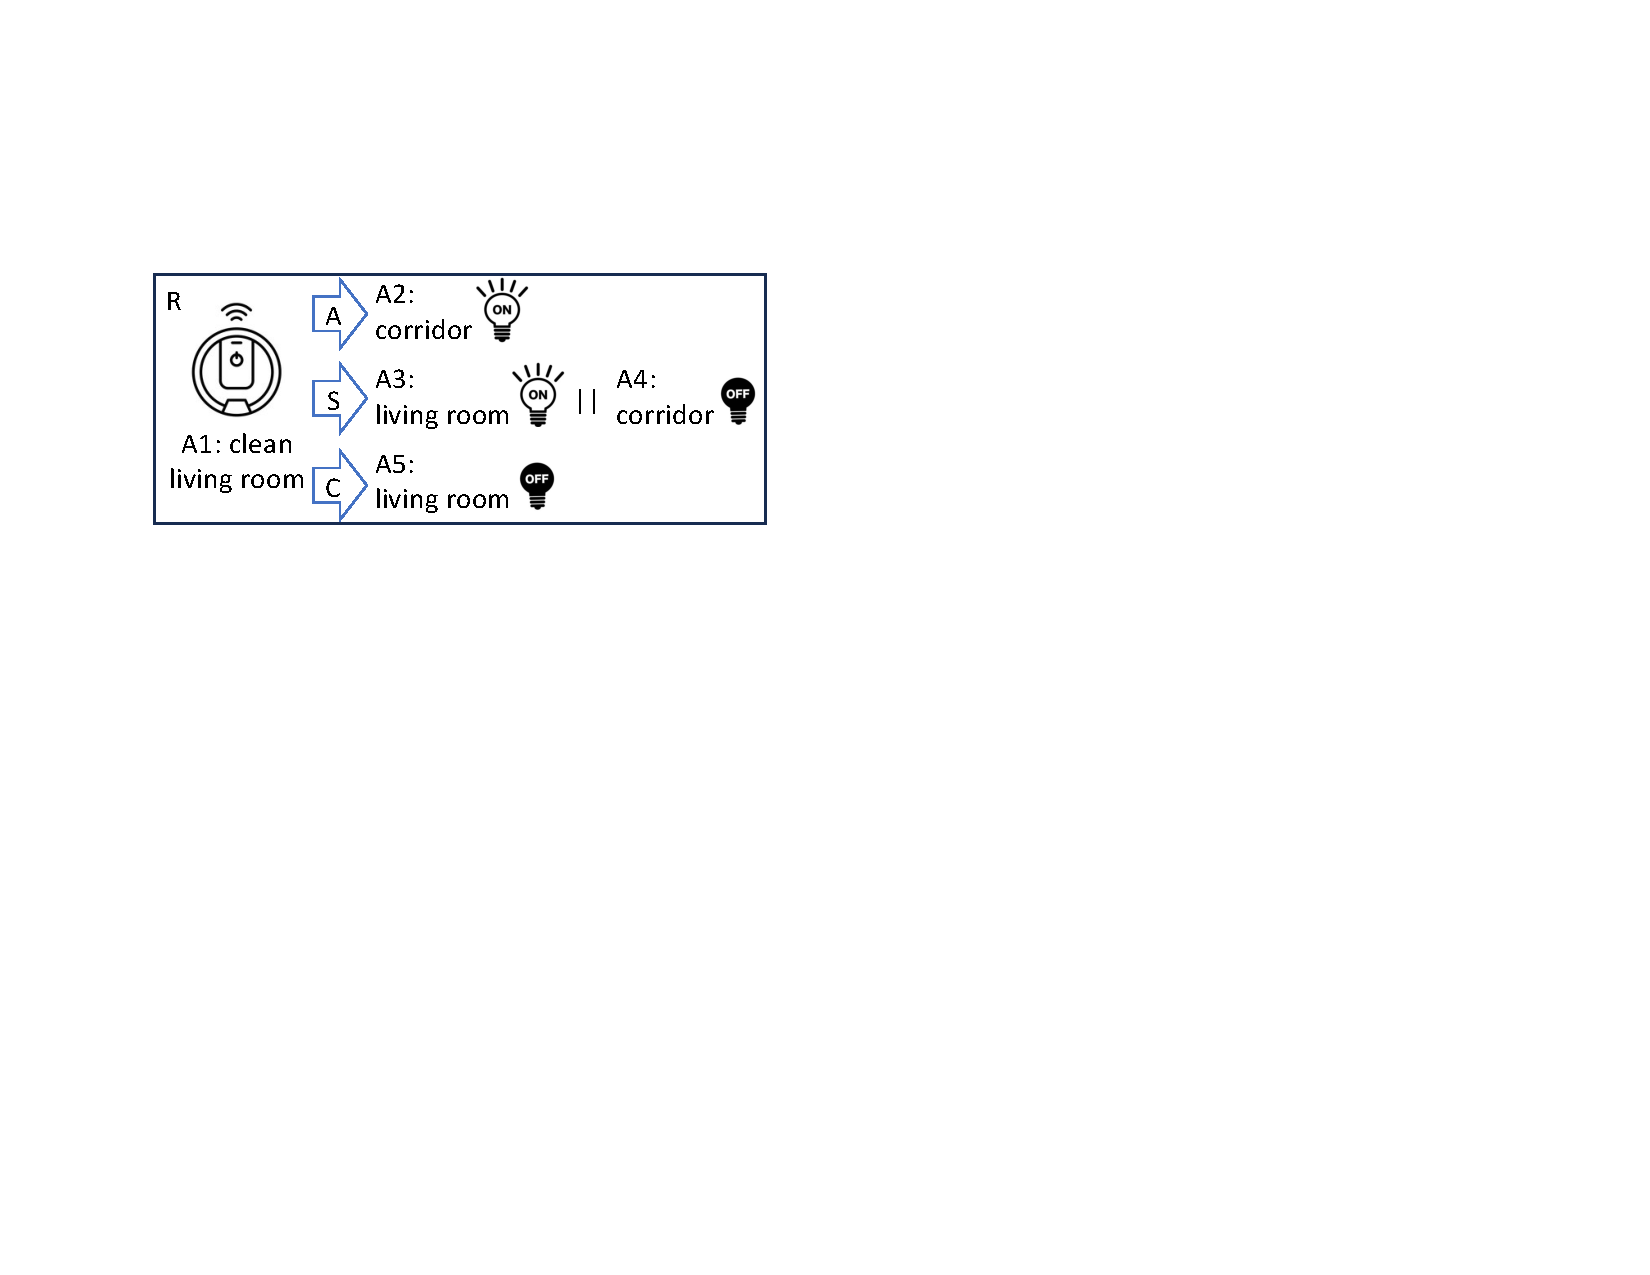
\includegraphics[width=0.5\textwidth]{RASC/figures/applications/energy-saving-vacuum-rasc.pdf}
        \caption{\small Single routine for energy-saving vacuum atop RASC.}
        \medskip
        \label{rasc:fig:energy-saving-vacuum-rasc}
    \end{subfigure}
    \begin{subfigure}[b]{\linewidth}
        \centering
        \vspace{0.2cm}
        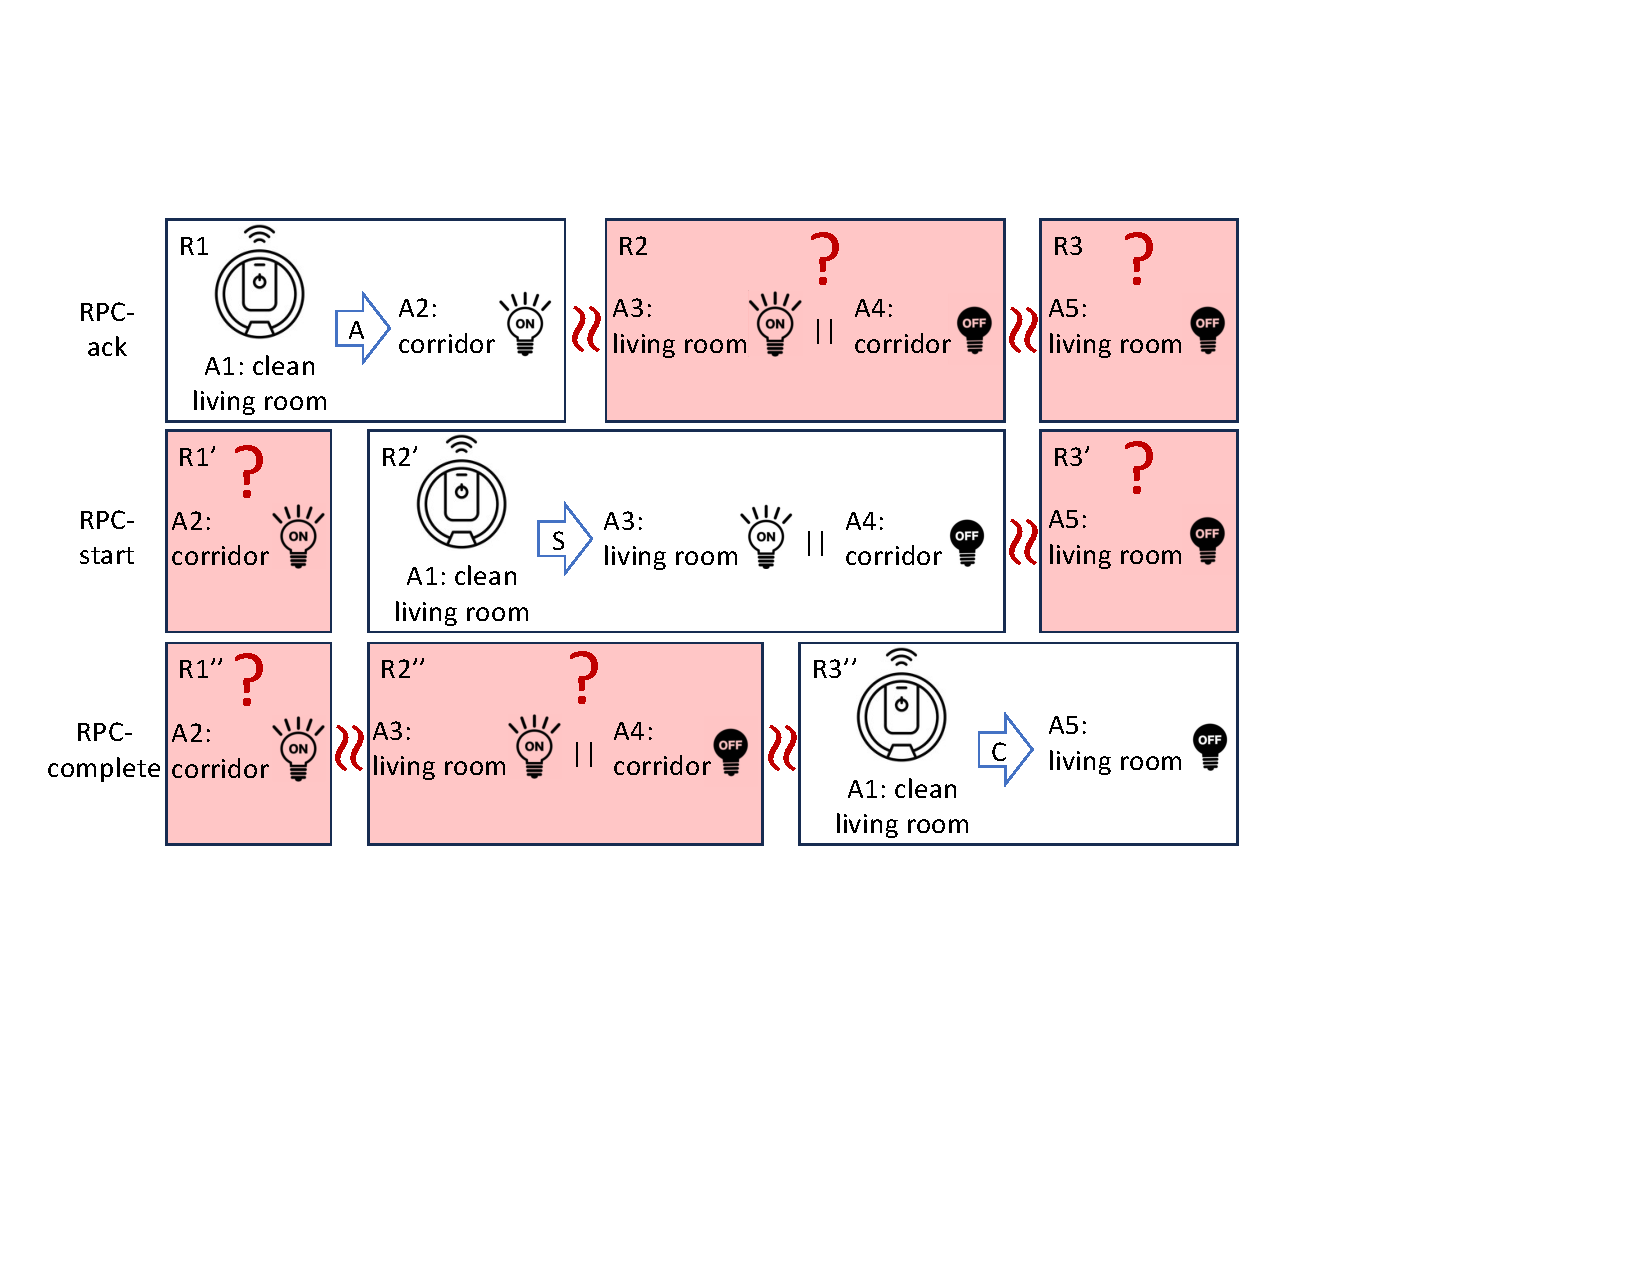
\includegraphics[width=0.9\textwidth]{RASC/figures/applications/energy-saving-vacuum-rpc.pdf}
        \caption{\small 
        Ineffective RPC-based energy-saving vacuum routines. Pink routines need complex---or unavailable---triggers (\textcolor{darkred}{?}; e.g., ``vacuum in living room'' $\land$ ``cleaning/returning''). With suboptimal triggers, cross-routine conflicts (\rotatebox{90}{\bf \textcolor{darkred}{$\approx$}}) arise or actions fire unintentionally.
        }
        \label{rasc:fig:energy-saving-vacuum-rpc}
    \end{subfigure}
    \caption{\bf \small Routine example with dependencies on \textit{Acknowledgment} (A), \textit{Start} (S) and \textit{Completion} (C) among actions. {\it The vacuum requires light to navigate.}  
    }
    \medskip
    \label{rasc:fig:energy-saving-vacuum}
\end{figure}

\noindent \textbf{Goals for an RPC Alternative: }
The inherent {\it one-shot} nature of an RPC is a mismatch with the {\it long-running} nature of IoT actions.  We posit that the call-response for IoT device actions must adhere to two inter-related principles: 
\noindent (1) \textbf{\textit{Observability}}: the ability to track a device action;
\noindent (2) \textbf{\textit{Programmability}}: the ability to write and efficiently run {\it expressive} programs.

Observability requires that the hub (or user device) receive \textbf{\textit{progress updates}} at critical action execution points. If any key action part fails, internal mechanisms must \textbf{\textit{detect failure fast}}, and mitigate. Second, programmability implies that programs support expressive and \textbf{\textit{diverse dependencies}} among actions (inside a program, and across programs), e.g., start the next action $A2$ earlier, {\it during} execution of a previous dependent action $A1$, after $A1$ has crossed key internal points (rather than waiting for $A1$ to finish). 
These dependencies require us to design \textbf{\textit{dynamic scheduling}} for concurrent smart-space actions. Rescheduling is vital because varying action lengths and tail latency (\Cref{rasc:fig:action-length-variability}) cause executions to deviate from original estimates and schedules.
This intertwined nature of observability and programmability---summarized in \Cref{rasc:tab:properties}'s four goals---parallels challenges
distributed systems~\cite{omnitable,viperprobe}, Kubernetes~\cite{kubern8observability}, and SDNs~\cite{simon}.

\noindent \textbf{A New Abstraction:}
This paper proposes {\it \abs} (Request-Ack-Start-Complete), a new abstraction for IoT devices, as an alternative to RPC. RASC does not replace RPC, but instead can be built atop RPC.
\abs{} provides Replies at three critical action lifecycle points: {\bf A}ck (the action is received by the device but not yet started), {\bf S}tart (the device starts the action), and {\bf C}omplete (the device finishes the action). Naturally, some of these replies may overlap   (e.g., if the action is short), but each is essential for longer actions 
to satisfy \Cref{rasc:tab:properties}'s goals.

Consider a robotic vacuum that requires ambient light in its work area (for the robot's camera).
\Cref{rasc:fig:energy-saving-vacuum-rasc} shows a routine (a program with a set of actions) named $R$ expressed with diverse action dependency types. {Because the vacuum needs light for its camera to navigate, initially the corridor light is switched on so that the vacuum can find its way to the living room (since the precondition for the action is that the vacuum reach the living room). After that, the living room light is kept on for vacuuming, but the corridor light is switched off. When the vacuum has completed and docks in the living room, the living room light is switched off. } 
Similar routines exist involving lawn-mowers~\cite{santhoshini2024implementation}, tele-presence robots~\cite{tsui2011exploring}, etc.  

\Cref{rasc:fig:energy-saving-vacuum-rpc} shows that to {\it correctly} implement $R$ via RPC variants, $R$ needs to be split into several routines. 
Each split is problematic because (i) there are no good triggers for the pink routines (e.g., vacuum location cannot be used in trigger clauses), and (ii) if users go for clauses provided by the APIs, which tend to be simple, they will not get the intended result. 

Our system \sysname{} implements the \abstraction{} abstraction. 
Assuring \Cref{rasc:tab:properties} entails several challenges. 
First, we have to build a {\bf progress/failure detector} atop \abs, that minimizes detection time while respecting device constraints.
For poll-only devices,
it must poll often enough to track progress and catch failures promptly without overwhelming devices.
Second, atop \abs{} when we provide support for expressive routine dependencies, we must innovate {\bf new dynamic scheduling algorithms} that reduce end-to-end latency (from routine arrival to completion).
Third, a key principle in our design is backwards compatibility: to make \sysname{} immediately deployable atop today's ecosystems, IoT devices and their vendor services cannot be modified. This forces us to work within the constraints of existing RPC interfaces. 
This is challenging as (i) \abs{} is more expressive than RPCs, and (ii) RPCs may go either via the IoT cloud service, or directly to the device.

This paper makes the following contributions:
\begin{itemize}
\item We present a new expressive RPC-enhancing abstraction called \abs, for IoT settings.
\item We build the \sysname{} system that implements \abs{} over existing RPC-based IoT APIs.
To support action progress updates and failure detection, we propose new techniques for efficient device polling. We also propose new dynamic scheduling policies for 
diverse action dependencies.
\item We integrate \sysname{}
with the popular and open-source home automation system called Home Assistant~\cite{HomeAssistant}.
\item We measured action execution times for various devices in office buildings. 
We use these and sets of real routines to perform trace-driven evaluation. We find that (i) \sysname{} 
detects completion within 2-13 RPCs and 2s-16s over 90\% of the time, and (ii) 
our routine scheduling policies outperform state-of-the-art by 10\%-55\%.

\end{itemize}
